% !TeX root = ../main.tex

\chapter{学位论文形式结构}

\section{字数要求}
\begin{enumerate}
    \item 硕士论文: 正文一般为$1 \sim 3$万字;
    \item 博士论文: 正文一般不超过$15$万字。
\end{enumerate}

\section{论文结构}
\begin{figure}
    \centering
    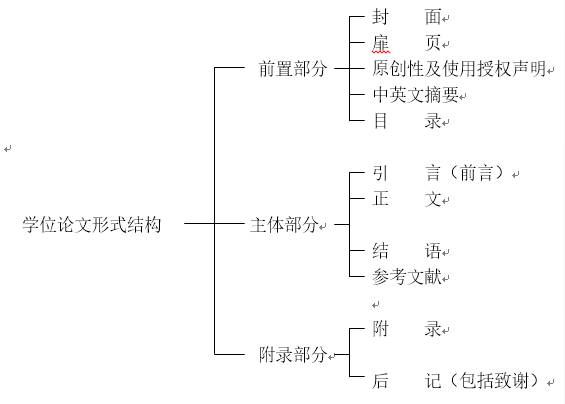
\includegraphics[width=.7\textwidth]{doc_structure.jpg}
    \caption{文档结构}
\end{figure}

\section{前置部分}


\begin{enumerate}
    \item 封面和封底:由研究生院统一印刷,封面内容一律打印,其中导师姓名以研究生院备案名单为准。\\
          题目:在25字以内,能简明、具体、确切地表达论文特定内容,必要时,可以使用副标题。中文、英文题目应一致。
      \item 扉页内容包括学位论文中文、英文题目、专业名称、申请人姓名、导师姓名及论文答辩委员会组成 (由答辩委员会成员签名)。
      \item 原创性及学位论文使用授权声明。
      \item 中英文摘要。
\end{enumerate}


\section{主体部分}
\begin{enumerate}
    \item 主体部分包括引言 (前言),国内外文献综述,正文, 结语,参考文献。要求图表清晰,叙述流畅,章节有序,层次 分明。\\
    引言 (前言)部分内容主要为本研究课题的学术背景及理论与实际意义;本研究课题的来源及主要研究内容;建立研究的线索与思路。

    \item 文中的图、表、公式等,一律用阿拉伯数字按章顺序编号。如图 1-1、图2-2, 表 1-1、表 2-1,公式 (1-1) 等。图序及图名置于图的下方,居中排列;表序及表名置于表的上方,居中排列。详见第\ref{figures_tables}章的说明。

    \item 参考文献
    \begin{enumerate}
        \item 参考文献为论文中所有引文、引用观点以及对论文有重要影响和启发的文献;
        \item 参考文献按在论文中出现的先后依次排序;个别学科若通用该学科惯用的排序规范,可以例外;
        \item 参考文献内容一般排列在论文末尾 (论文篇幅较大且引用文献较多的,可在每章末尾注出),序码与论文加注处对应;
        \item 参考文献标注格式: 使用国标GB/T 7714-2015标准, 建议使用工具自动控制引文格式, 
        以保证格式规范。
        该\LaTeX{}模板已经对引文格式做了配置,
        用户需要将所需参考文献的信息存在 \texttt{bib} 格式的文件\texttt{ref/refs.bib}中, 
        通过 \verb|\cite{}|命令在恰当位置引用 (详见第\ref{citations}章的说明)。
        \texttt{bib}文件可从文献管理工具导出或自己用 \texttt{JabRef} 等软件编辑。
    \end{enumerate}

    \item 注释:可以用 “脚注”或 “文后注”来标注引用著作中的一些观点和案例,但全文标注方式应统一。
\end{enumerate}

\section{附录部分}
\begin{enumerate}
    \item 附录\\
        附录是正文主体的补充。下列内容可以作为附录:
        \begin{enumerate}
            \item 攻读学位期间发表的 (含已录用,并有录用通知书的)与学位论文相关的学术论文目录 。
            \item 由于篇幅过大,或取材于复制件不便编入正文的材料、数据。
            \item 对本专业同行有参考价值,但一般读者不必阅读的材料。
            \item 论文中使用的符号意义、单位缩写、程序全文及有关说明书。
            \item 附件:计算机程序清单、软磁盘、鉴定证书、获奖 奖状或专利证书的复印件等。
        \end{enumerate}
    \item 后记\\
        后记是有关本论文情况的说明性文字,主要是交代编写过程,阐述作者的感想和体会,对有关单位或个人的致谢语等。
\end{enumerate} 


\cleardoublepage
